% Delete this, if you do not want the table of contents to pop up at
% the beginning of each subsection:
% \AtBeginSubsection[]
% {
% 	\begin{frame}<beamer>{Sumário do capítulo}
% 		% \tableofcontents[currentsection,currentsubsection]
% 		% \tableofcontents[currentsection, hideothersubsections,sectionstyle=show/shaded,]
%         \tableofcontents[sectionstyle=show/hide,subsectionstyle=show/show/hide]
% 	\end{frame}
% }


% \setcounter{tocdepth}{1} % Show sections
% \setcounter{tocdepth}{2} % + subsections
% Title page frame
\begin{frame}
    \begin{tikzpicture}[remember picture,overlay]
        \node[above right, inner xsep=0pt, inner ysep=0pt] at (current page.south west)
        {
            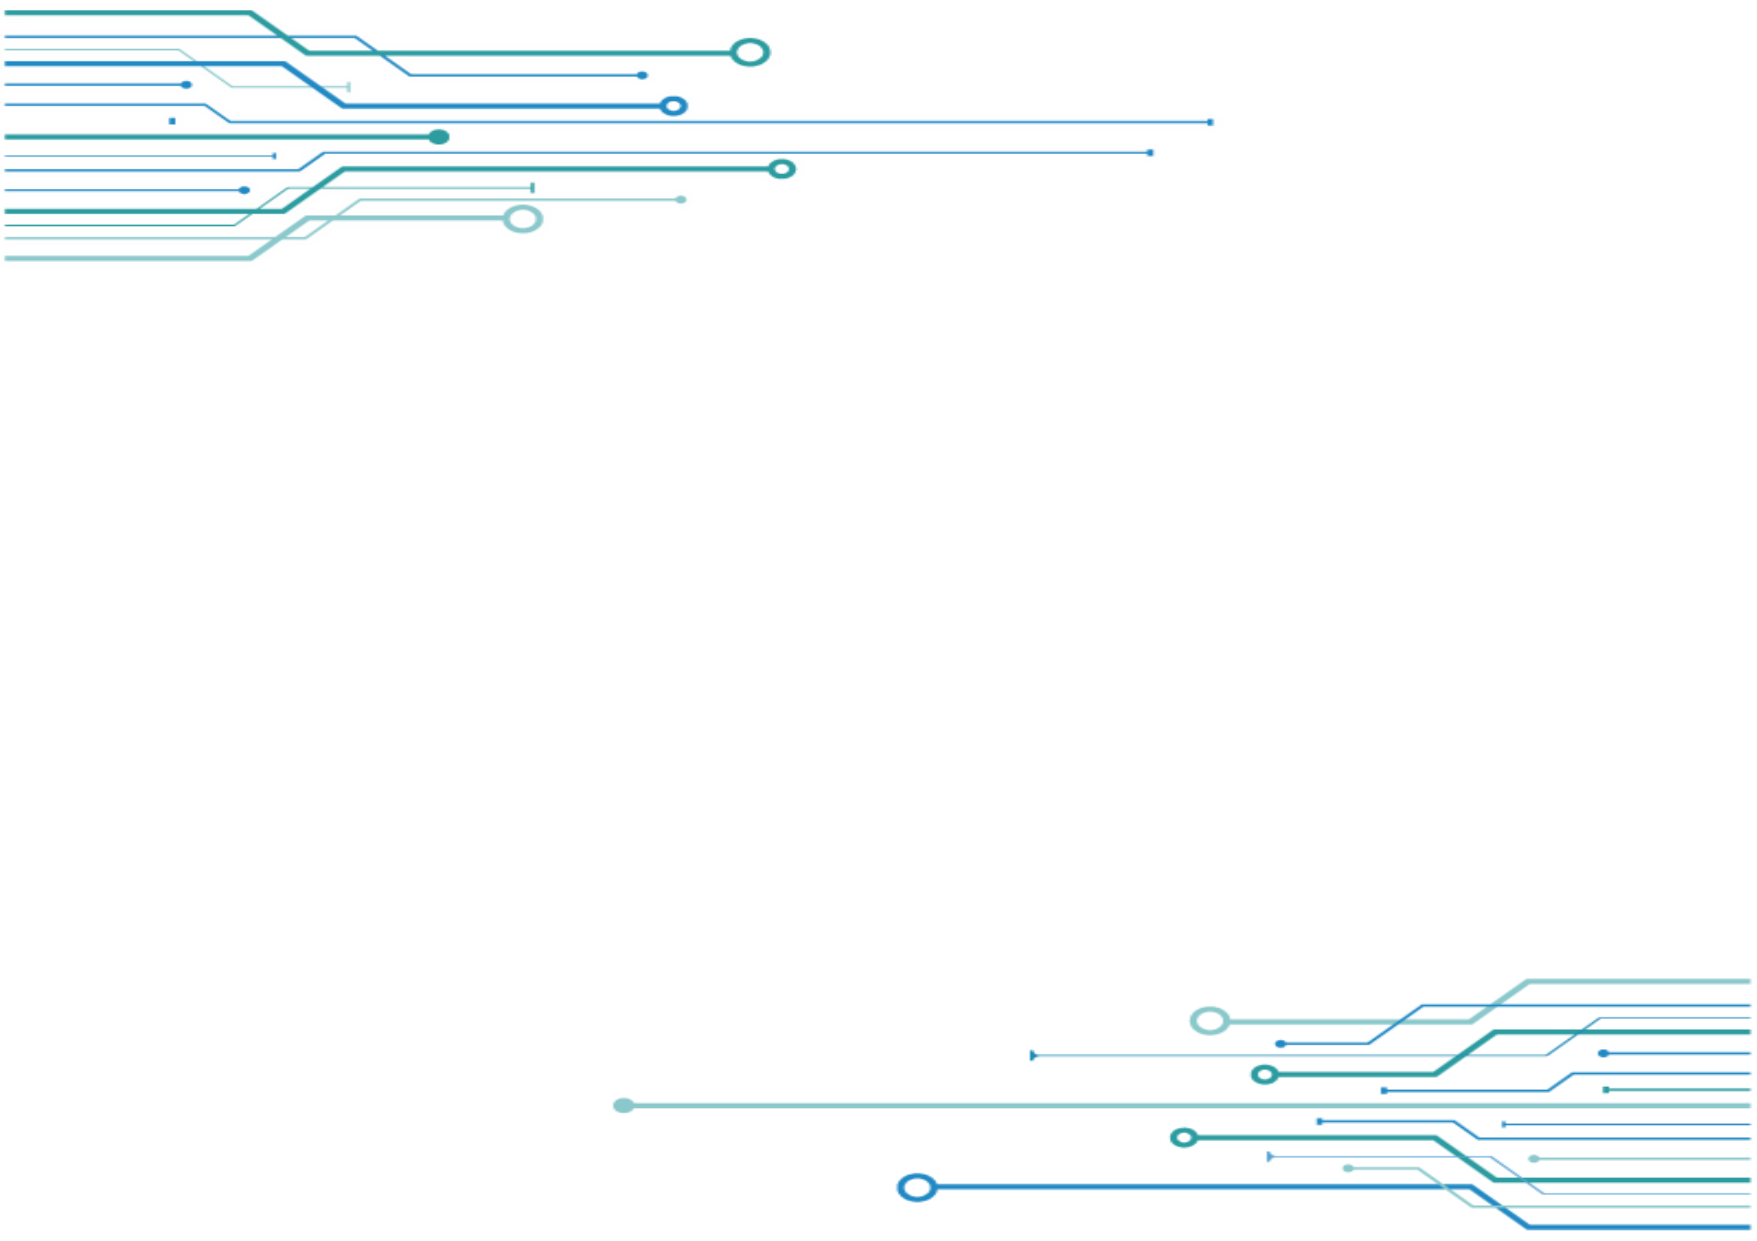
\includegraphics[width=\paperwidth]{back34.png}
        };
    \end{tikzpicture}
    \titlepage
    \tikz [remember picture, overlay] %
    \node [shift={(0.1cm,1.4cm)}] at (current page.south west) %
    [anchor=north west] %
    {
\includegraphics[height=0.9cm]{UNIFAP.png}};
\end{frame}

% Remove logo from the next slides
\logo{}

% Outline frame
\begin{frame}[t]{Sumário}
    \begin{tikzpicture}[remember picture,overlay]
        \node[above right, inner xsep=0pt, inner ysep=-20pt] at (current page.south west)
        {
            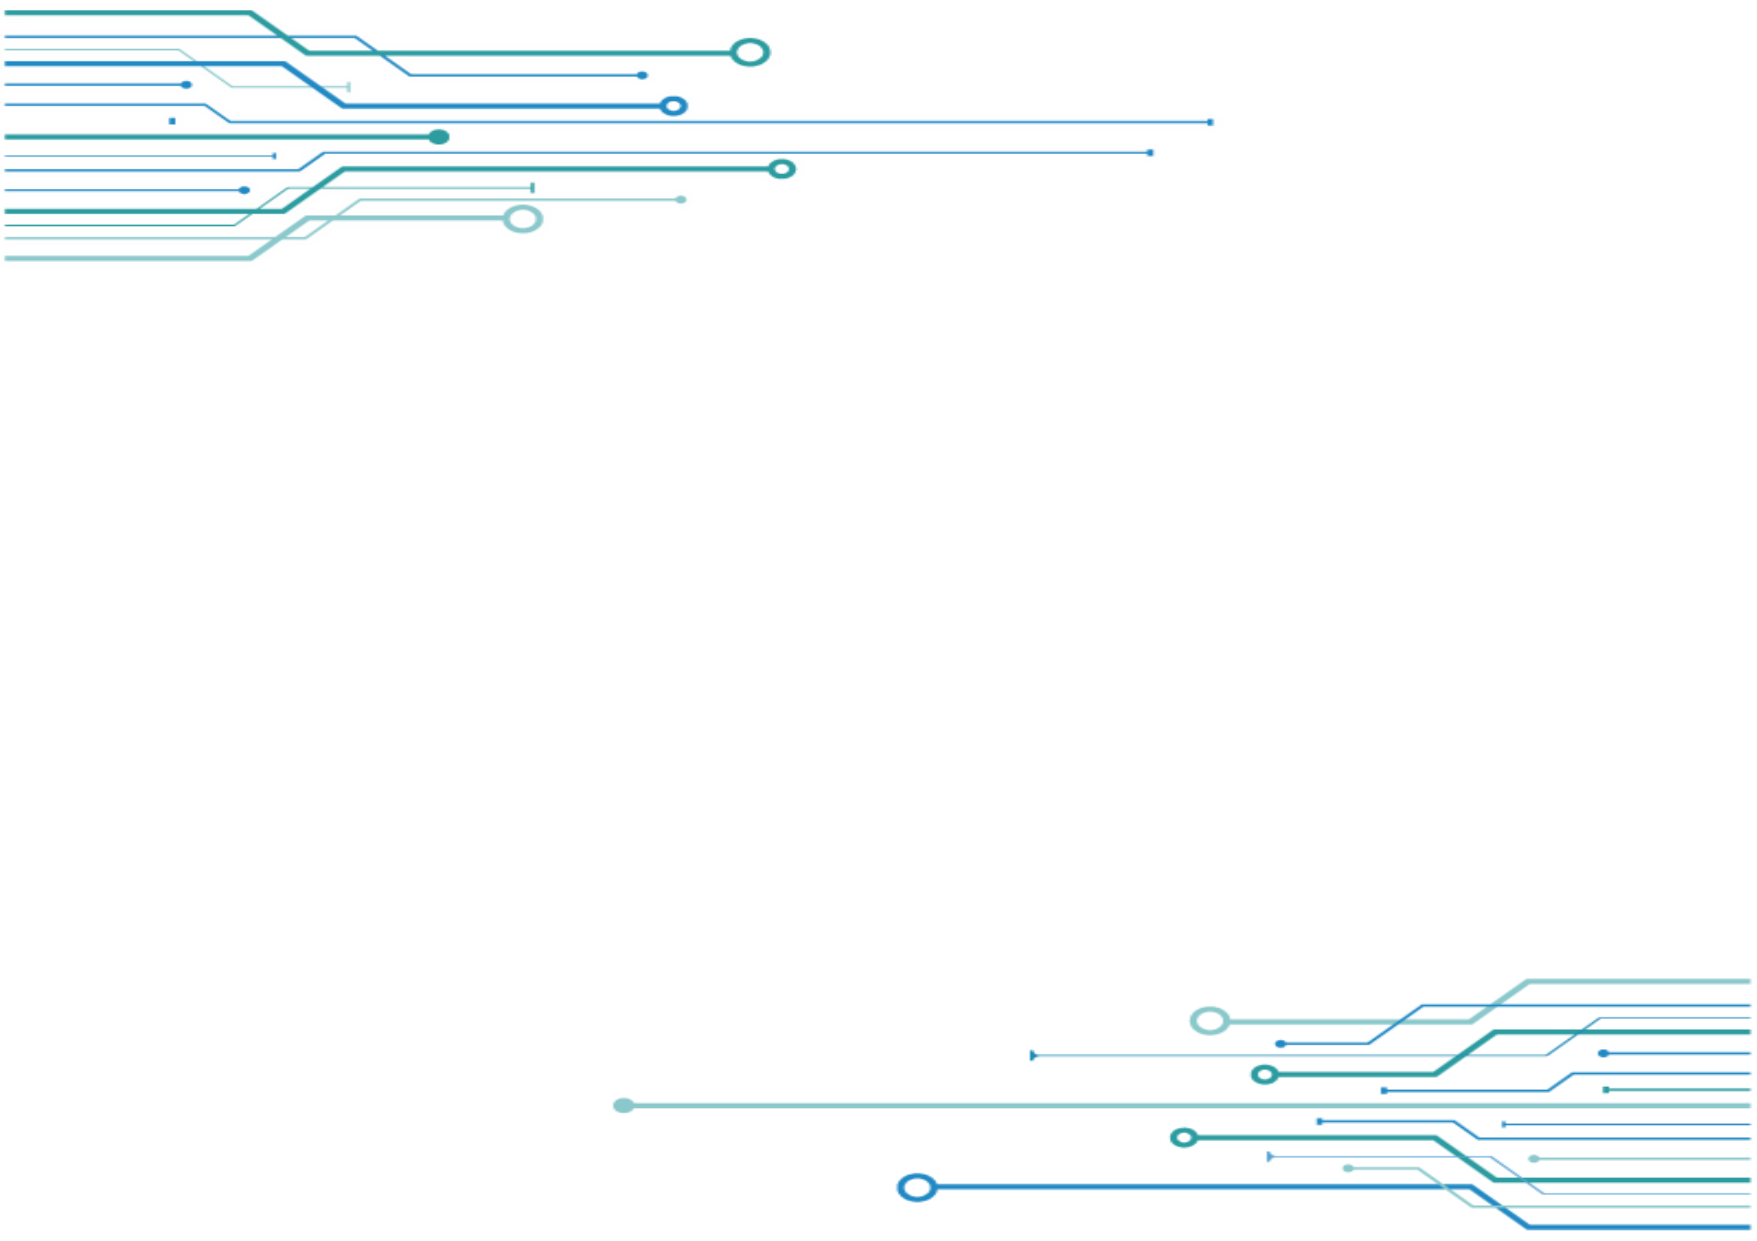
\includegraphics[width=\paperwidth]{back34.png}
        };
    \end{tikzpicture}
    \tableofcontents[sections={1-3}]
\end{frame}
%
% \begin{frame}[t]{Sumário}
%     \tableofcontents[sections={4-}]
% \end{frame}
